\part{Introduzione}
\makepart

\begin{frame}
    \frametitle{Massa dell'assione}
    {\color{fzjblue} Una nuova particella}
    \begin{itemize}
        \item L'assione è un'ipotetica particella elementare
        \item È descritta dal modello di Peccei-Quinn
        \item Introdotto per spiegare la piccola violazione CP della QCD
        \item Solo in seguito Weinberg e Wilczek capirono l'importanza dell'assione
    \end{itemize}
    {\color{fzjblue} Materia oscura?}
    \begin{itemize}
        \item L'assione ha un accoppiamento molto debole con le altre particelle
        \item È il principale candidato ad essere materia oscura
    \end{itemize}
\end{frame}

\begin{frame}
    \frametitle{Lagrangiana efficace}
    \begin{itemize}
        \item L'assione è accoppiato a un'altra particella: il s-assione
        \item Sono descritti dal campo scalare complesso $\phi$
            \begin{itemize}
                \item $\left|\phi\right|$ è il campo del s-assione
                \item $\arg\phi$ è il campo dell'assione
            \end{itemize}
        \item La lagrangiana è:
        $$\mathcal{L} = \partial_\mu\phi^*\partial^\mu\phi%
                      - \frac{\lambda}{8}\left(\phi^*\phi-f_a^2\right)%
                      + \chi_t\frac{\left|\phi\right|}{f_a}\cos\arg\phi$$
    \end{itemize}
\end{frame}

\begin{frame}
    \frametitle{Cappello messicano}
    Il potenziale efficace è:
            $$V = \frac{\lambda}{8}\left(\phi^*\phi-f_a^2\right)^2 -%
            {\color{fzjred} \chi_t\frac{\left|\phi\right|}{f_a}\cos\arg\phi}$$
    \begin{center}
        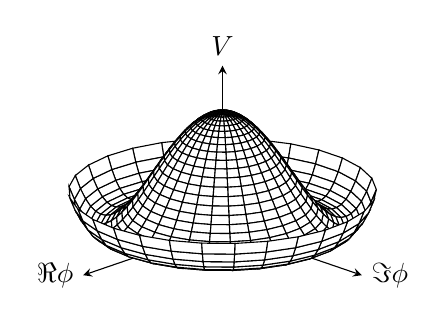
\begin{tikzpicture}
            \begin{axis}
            [
                width = 0.65\textwidth,
                height = 0.65\textwidth,
                axis equal image,
                view={135}{20},
                ticks=none,
                axis lines = center,
                xmax = 1.6,
                ymax = 1.6,
                zmax = 1.4,
                x label style={anchor=east},
                y label style={anchor=west},
                z label style={anchor=south},
                xlabel=$\Re\phi$,
                ylabel=$\Im\phi$,
                zlabel=$V$,
                samples=30,
                domain=0:360,
                y domain=0:1.25, clip=false,
            ] \addplot3 [surf, shader=flat, draw=black, fill=white, z buffer=sort]
                ({cos(x)*y}, {sin(x)*y}, {(y^2-1)^2});
            \end{axis}
        \end{tikzpicture}%
        \hspace{0.05\textwidth}%
        \begin{tikzpicture}
            \begin{axis}
            [
                width = 0.65\textwidth,
                height = 0.65\textwidth,
                axis equal image,
                view={135}{20},
                ticks=none,
                axis lines = center,
                xmax = 1.6,
                ymax = 1.6,
                zmax = 1.4,
                x label style={anchor=east},
                y label style={anchor=west},
                z label style={anchor=south},
                xlabel=$\Re\phi$,
                ylabel=$\Im\phi$,
                zlabel=$V$,
                samples=30,
                domain=0:360,
                y domain=0:1.25, clip=false,
            ] \addplot3 [surf, shader=flat, draw=fzjred, fill=white, z buffer=sort]
                ({cos(x)*y}, {sin(x)*y}, {(y^2-1)^2 - 0.2*y*cos(x)});
            \end{axis}
        \end{tikzpicture}
    \end{center}
\end{frame}

\begin{frame}
    \frametitle{Osclillazioni massive}
    \begin{itemize}
        \item Sono presenti due modi di oscillazione
        \item Le loro masse corrispondenti sono:
            \begin{itemize}
                \item s-assione: $m_s \sim \sqrt\lambda\,f_a$
                \item assione: $m_a \sim \sqrt\chi_t/f_a$
            \end{itemize}
        \item $f_a$ determina l'ordine di grandezza di $m_s$
        \item $f_a$ è molto grande: $\sim 10^{10}\ \text{GeV}$
        \item $\chi_t$ è l'accoppiamento, ed è molto piccolo
        \item La massa dell'assione è anch'essa molto piccola
    \end{itemize}
\end{frame}

\begin{frame}
    \frametitle{Come si calcola la massa dell'assione}
    Si definisce un funzionale chiamato {\color{fzjblue} carica topologica}:
    $$Q = \frac{g^2}{16\pi^2}\int\mathrm{d}^4x\,%
    \epsilon_{\mu\nu\rho\sigma}F_{\mu\nu}F_{\rho\sigma}$$
    \begin{itemize}
        \item $F_{\mu\nu}$ è il tensore degli sforzi del campo gluonico
        \item $Q$ assume solo valori interi nei sistemi comunemente considerati
        \item $Q$ è utile perché la sua suscettibilità è proporzionale a $m_a$:
            $$\frac{\left<Q^2\right>}{V}=\chi_t=f_a^2\,m_a^2$$
        \item È possibile ottenere $m_a$ misurando $Q$ %
            e mediando il quadrato sulle configurazioni di campo
    \end{itemize}
\end{frame}

